\documentclass[11pt]{article}
\usepackage[T1]{fontenc}
\usepackage[utf8]{inputenc}
\usepackage[portuguese]{babel}
\usepackage{amsmath}
\usepackage{graphicx}
\usepackage{float}
\usepackage{enumitem}

\graphicspath{{}}

\newcommand{\numpy}{{\tt numpy}}

\topmargin -.5in
\textheight 9in
\oddsidemargin -.25in
\evensidemargin -.25in
\textwidth 7in

\begin{document}

\author{Lucas Emanuel Resck Domingues}
\title{Aula prática 4
\medbreak
\large Método dos mínimos quadrados}
\maketitle

\medskip

\begin{enumerate}

\item 

\begin{enumerate}
    \item Queremos aproximar uma reta $y = a + bx$. Considerando 1900 como $t = 0$, ficamos com o seguinte sistema:
    
$$\begin{cases}
a + 20b = 54,1\\
a + 30b = 59,7\\
a + 40b = 62,9\\
a + 50b = 68,2\\
a + 60b = 69,7\\
a + 70b = 70,8\\
a + 80b = 73,7\\
a + 90b = 75,4
\end{cases}$$

Temos as matrizes $A$ e $b$:

$$A = \begin{bmatrix}
1&20\\
1&30\\
1&40\\
1&50\\
1&60\\
1&70\\
1&80\\
1&90
\end{bmatrix}\textrm{, }
b = \begin{bmatrix}
54,1\\
59,7\\
62,9\\
68,2\\
69,7\\
70,8\\
73,7\\
75,4
\end{bmatrix}$$

A solução para o método dos mínimos quadrados, como visto em aula, é $\mathbf{x}$ tal que
$$A^TA\mathbf{x}=A^Tb$$
Resolvendo computacionalmente (via Scilab), obtemos $\mathbf{x} = (a, b) \approx (50,82; 0.29)$. Para $x = 100$ (referente ao ano $2000$), obtemos $y = 79,9$.
\bigbreak
\item A expectativa de vida nos Estados Unidos em 2000 foi $76,64$. Isso mostra que nosso modelo não é muito preciso... Uma possível justificativa para isso é que o crescimento da população não é linear, como tentamos modelar.

\end{enumerate}

\item

\begin{enumerate}
    \item Queremos aproximar $s(t) = s_0 + v_0t + \frac{1}{2}gt^2$. Formemos $A$ e $b$:

    $$A = \begin{bmatrix}
    1& 0,5& 0,25\\
    1& 1& 1\\
    1& 1,5& 2,25\\
    1& 2& 4\\
    1& 3& 9
    \end{bmatrix}\textrm{, }
    b = \begin{bmatrix}
    11\\
    17\\
    21\\
    23\\
    18
    \end{bmatrix}$$
    
    Resolvendo $A^TA\mathbf{x}=A^Tb$, obtemos $\mathbf{x} = (s_0, v_0, \frac{g}{2}) \approx (1,92; 20,31; -4,97)$. Veja que $g \approx -9,94 \approx -9,81  \textrm{m/s}^2$, realmente.
    \bigbreak
    \item $s_0 \approx 1,92 \textrm{m}$, $v_0 \approx 20,31\textrm{m/s}$ e $g \approx -9,94 \textrm{m/s}^2$.
    \bigbreak
    \item Basta resolver $0 = s_0 + v_0t + \frac{1}{2}gt^2$. Então $t\approx 4,18 \textrm{s}$.
    \bigbreak
\end{enumerate}

\item 

\begin{enumerate}
    \item 
    Queremos aproximar $y = p(t) = ce^{kt}$. Podemos aproximar $\ln y = \ln c + kt$, um modelo linear. Então $\mathbf{x} = (\ln c, k)$. Calculamos $b$ aplicando $\ln$ nas populações. Utilizando a função \textbf{Gaussian\_Elimination\_4}, da aula prática 1, para a resolução do sistema e considerando $t=0$ para $1950$, temos:

    \begin{figure}[H]
        \centering
        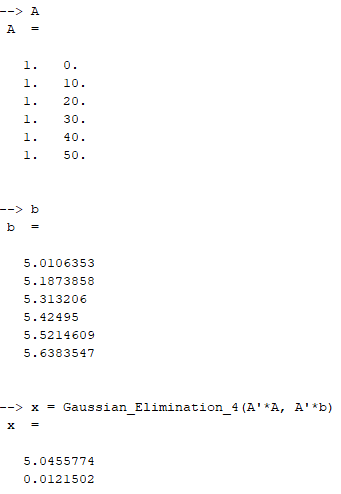
\includegraphics[]{3-a}
        \caption{Matrizes $A$ e $b$ e resolução do sistema $A^TA\mathbf{x}=A^Tb$.}
    \end{figure}
    
    A partir disso, concluímos que $c \approx e^{5,04} \approx 155,33$ e $k \approx 0,01$. Portanto, $p(t)\approx155,33e^{0,01t}$. Sendo assim, a taxa de crescimento é $p'(t) \approx 1,89e^{0,01t}$.
    \bigbreak
    \item A população estimada dos EUA em 2010 é $p(60) = ce^{k60} \approx 322,01$ milhões de pessoas. Em 2010, a população dos EUA foi de $309,3$ milhões de pessoas. Nosso modelo superestimou a população. Sabemos que um modelo exponencial também se adequa muito bem a um crescimento populacional de uma população já grande.
    \bigbreak
\end{enumerate}

\item

\begin{enumerate}
    \item Queremos aproximar $y = a + bx + cx^2$. Considerando 1970 como $t = 0$, temos:

    \begin{figure}[H]
        \centering
        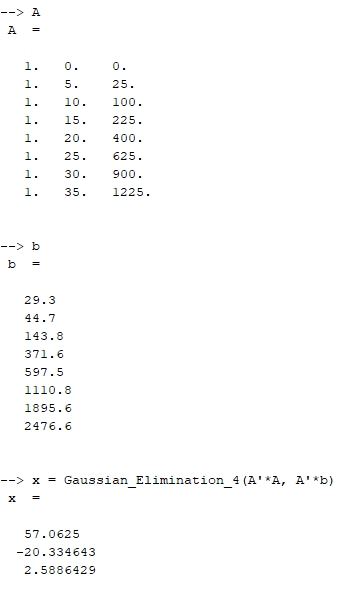
\includegraphics[]{4-a}
        \caption{Matrizes $A$ e $b$ e resolução do sistema $A^TA\mathbf{x}=A^Tb$.}
    \end{figure}
    
    Portanto, $y \approx 57,06 - 20,33x + 2,59x^2$
    \bigbreak
    \item Queremos $y = ce^{kt} \iff \ln y = \ln c + kt$. Aplicamos $\ln$ nas médias salariais e temos:

    \begin{figure}[H]
        \centering
        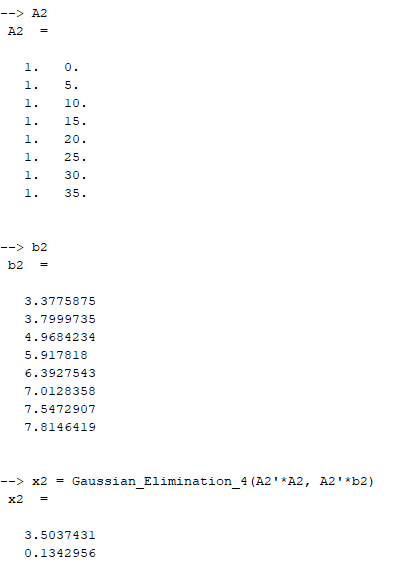
\includegraphics[]{4-b}
        \caption{Matrizes $A$ e $b$ e resolução do sistema $A^TA\mathbf{x}=A^Tb$.}
    \end{figure}
    
    Ficamos com $y \approx e^{3,50}e^{0,13t} \approx 33,12e^{0,13t}$.
    \bigbreak
    \item O erro é dado por $e = b-Ax$. No caso do modelo exponencial, como aplicamos $\ln$, devemos antes calcular os exponenciais dos valores em $b$ e em $Ax$. Calculamos as normas dos erros dos modelos quadrático e exponencial, respectivamente:

    \begin{figure}[H]
        \centering
        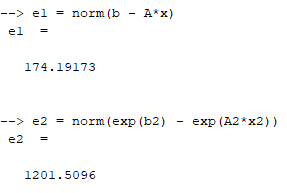
\includegraphics[]{4-c}
        \caption{Normas dos erros dos modelos quadrático e exponencial, respectivamente.}
    \end{figure}
    
    Vemos que o modelo quadrático se ajustou melhor aos dados.
    \bigbreak
    \item Utilizando a aproximação quadrática e calculando computacionalmente: em 2010, estimamos um salário de $3385,5$ milhares de dólares e, em 2015, $4384,0$.
\end{enumerate}

\item No Scilab, lemos o arquivo \textbf{cancer\_train.csv} utilizando a função \textbf{csvRead()}. Seja $\mathbf{w} = (c_0, c_1, \ldots, c_{10})$. Formamos a matriz $A$ com as dez primeiras colunas de $cancer\_train$ (com os vetores $\mathbf{x}$ das características dos pacientes), adicionando uma primeira coluna com elementos $1$. $b$ é a matriz com a última coluna de $cancer\_train$. Para encontrar o hiperplano que melhor se ajusta aos dados, resolvemos o sistema $A^TA\mathbf{w}=A^Tb$ computacionalmente:

\begin{figure}[H]
    \centering
    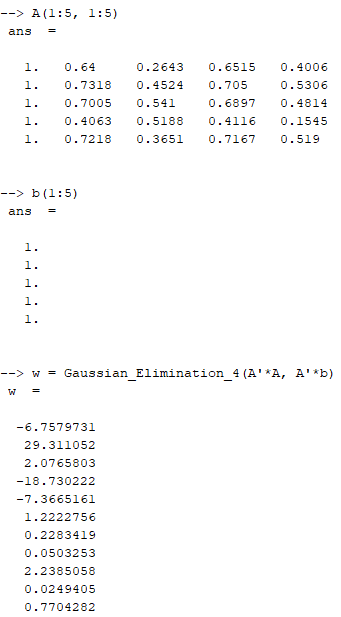
\includegraphics[]{5-1}
    \caption{Matrizes $A$ e $b$ e vetor $\mathbf{w}$}
\end{figure}

Observe que o elemento $z_i$ de $A\mathbf{w}$ é resultado do produto escalar de $A_i$ (linha $i$ de $A$) por $\mathbf{w}$. $z_i$ indica se a paciente $i$ tem ($z_i \ge 0$) ou não tem ($z_i < 0$) câncer de mama. Se multiplicarmos esse valor pelo resultado que já sabemos ($1$ ou $-1$), saberemos se o modelo acertou: se o produto for positivo, os dois valores têm mesmo sinal e o modelo acertou; caso contrário, o modelo errou. Ainda mais, podemos calcular o produto escalar entre $A\mathbf{w}$ e $b$, contar os acertos e calcular a porcentagem de acertos do modelo.

Para nosso arquivo de treinamento, o modelo obteve $93\%$ de acertos:

\begin{figure}[H]
    \centering
    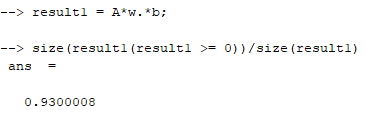
\includegraphics[]{5-2}
    \caption{Cálculo da porcentagem de acertos do modelo para o arquivo de treinamento.}
\end{figure}

Ou seja, nosso modelo se ajusta bem aos dados de treinamento.

Agora vamos ver se o modelo prevê bem para os dados de testes:

\begin{figure}[H]
    \centering
    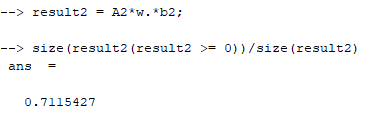
\includegraphics[]{5-3}
    \caption{Cálculo da porcentagem de acertos do modelo para o arquivo de testes.}
\end{figure}

Obtemos $71\%$ de acertos. É um resultado razoável. Isso mostra que o modelo tem uma boa capacidade de generalização.

Vamos observar agora alguns resultados do modelo:

\begin{table}[H]
    \centering
    \begin{tabular}{|c||c|c|}
    \hline
                            & Treinamento       & Testes            \\
    \hline \hline
    Verdadeiros positivos   & $135$ ($45\%$)    & $60$ ($23\%$)     \\
    \hline
    Verdadeiros negativos   & $144$ ($48\%$)    & $125$ ($48\%$)    \\
    \hline
    Falsos positivos        & $10$ ($3,33\%$)   & $75$ ($28,8\%$)   \\
    \hline
    Falsos negativos        & $11$ ($3,67\%$)   & $0$ ($0\%$)       \\
    \hline
    \end{tabular}
    \caption{Resultados do modelo.}
\end{table}

Nos resultados para os dados de treinamento, observamos que tanto os acertos quanto os erros não dependem muito se a paciente tem ou não câncer de mama. Além disso, o modelo obtém uma razoável razão de acertos.

Porém, para os dados de testes, obtemos algo curioso: $0$ falso negativo. Isso é, para $0$ paciente com câncer de mama o modelo apontou que não havia câncer. E isso sem que o modelo apontasse todas as pacientes com câncer de mama, ou seja, sem que ele tivesse uma quantidade exorbitante de falsos positivos.

Na verdade, a razão de falsos positivos aumentou bastante em relação aos dados de testes, mas ainda assim o modelo é regular.

\end{enumerate}
\end{document}
\grid
\grid